\documentclass[conference]{IEEEtran}

\usepackage{cite}
\usepackage{amsmath,amssymb}
\usepackage{booktabs}
\usepackage{array}
\usepackage{tabularx}
\usepackage{url}
\usepackage{graphicx}
\usepackage{float}
\usepackage{placeins}
\usepackage{xcolor}
\newcommand{\chg}[1]{{\color{blue}#1}}

\setlength{\textfloatsep}{4pt plus 1.0pt minus 1.0pt}
\setlength{\floatsep}{3pt plus 1.0pt minus 1.0pt}
\setlength{\intextsep}{3pt plus 1.0pt minus 1.0pt}
\setlength{\abovecaptionskip}{2pt}
\setlength{\belowcaptionskip}{2pt}

\title{Phoenix: Deterministic Self-Healing and Fault Tolerance for Autonomous Desktop Automation}

\author{
\IEEEauthorblockN{
Ramani G\textsuperscript{1},
Akshitha V G\textsuperscript{2},
Kruthin Shanmuk Yadav CG\textsuperscript{3},
Dhanyashree G V\textsuperscript{4},
Kaushal K\textsuperscript{5}
}
\IEEEauthorblockA{
Department of Computer Science and Engineering (AI \& ML)\\
AMC Engineering College, Bengaluru, Karnataka, India\\
Emails: gowrisan.ramani@amceducation.in, akshithavg1@gmail.com, \\
kruthin008@gmail.com, dhanyashreegv206@gmail.com, kaushalk123000@gmail.com
}
}

\begin{document}

\maketitle

\begin{abstract}
Reliable execution in multi-agent desktop automation requires robust error mitigation beyond raw task scheduling. Real-world workflows routinely encounter application crashes, missing file dependencies, transient network timeouts, and unauthorized operations. Existing agent recovery approaches rely on generative model reflection and replanning, which introduce inference latency, token cost, and potential decision variability. In this paper, we present the self-healing subsystem of Phoenix Agents, a deterministic, bounded recovery framework designed to diagnose and remediate execution exceptions in multi-agent desktop workflows without requiring an active Large Language Model during the recovery loop. The recovery mechanism is structured into five operational stages: error parsing, root-cause classification, strategy selection, patch generation, and retry execution. Recovery decisions follow typed contract assertions, deterministic rules, and a fixed retry budget ($K_{\text{max}} = 3$). \chg{Empirical evaluation across controlled fault injections demonstrates that the pipeline recovered 100.0\% of recoverable-by-design faults, safely rejected all non-recoverable faults, and achieved an overall recovery rate of 60.0\% (outperforming naive retry and fail-fast baselines), with an average recovery handling latency of 11.99~ms on mocked adapters.}
\end{abstract}

\begin{IEEEkeywords}
Phoenix Agents, Self-Healing, Multi-Agent Systems, Desktop Automation, Fault Recovery, Deterministic Recovery, Error Mitigation.
\end{IEEEkeywords}

\section{Introduction}
Multi-agent desktop and browser automation frameworks orchestrate complex workflows across web browsers, native applications, operating system terminals, and local file systems~\cite{bajoria2026}. However, executing tasks across heterogeneous host environments inherently exposes software agents to dynamic execution failures, such as transient network timeouts, missing file dependencies, altered DOM locators, process crashes, and permission denials.

In conventional script-based automation systems (e.g., Selenium, AutoHotkey), a single runtime exception causes catastrophic workflow failure. While recent research explores self-healing via Large Language Models (LLMs)---such as reflective prompt loops and continuous model replanning---each LLM call in recovery incurs latency and token cost that depend on the model and prompt size, along with safety risks from uncontrolled retries~\cite{babu2026,jeong2026}.

To address these challenges, we present the deterministic self-healing architecture of Phoenix Agents. Phoenix Agents uses an in-process asynchronous publish--subscribe EventBus for event delivery, while the five recovery stages execute sequentially within the recovery handler. The framework uses a lightweight 5-stage pipeline (Error Parsing, Root-Cause Analysis, Strategy Selection, Patch Generation, and Retry Execution) that diagnoses and remediates execution errors without requiring an active LLM runtime during error recovery.

The Primary Technical Contributions of This Paper:
\begin{itemize}
    \item \textbf{Structured 5-Stage Pipeline:} Modular in-process recovery executing error parsing, root-cause diagnosis, strategy selection, patch generation, and retry dispatch without LLM inferencing.
    \item \textbf{Deterministic In-Process Recovery Loop:} Rule-based mitigation policies and typed contract assertions achieving millisecond-scale handling latency \chg{($T_R = 11.99$~ms, $T_{\text{rec}} = 12.00$~ms on mocked adapters; 1.89~ms on real filesystem)}.
    \item \textbf{Bounded Retry \& Safety Guard Policy:} Strict enforcement of retry limits ($K_{\text{max}} = 3$) paired with safe rejection of non-recoverable operations.
    \item \chg{\textbf{Empirical Verification Across 125 Controlled Trials:} Benchmark evaluation demonstrating complete recovery on recoverable faults, zero safety violations, and significant advantage over naive retry and fail-fast baselines.}
\end{itemize}

\section{Related Work}

\subsection{Related Work and Differentiation}
\chg{\textbf{Foundations in Classic Fault Tolerance:} Phoenix Agents builds upon classical principles of dependable computing. Avi\v{z}ienis et al.~\cite{avizienis2004} formalized the fundamental taxonomy of faults, errors, and failures, establishing the necessity of error detection and system recovery boundaries. In high-availability systems, Gray and Siewiorek~\cite{gray1991} demonstrated that transient software faults can be overcome through modular process isolation and bounded restart mechanisms. In enterprise software architecture, Nygard~\cite{nygard2018} formalized stability patterns including circuit breakers, bounded retries, and exponential backoff to prevent cascading failures. For multi-step distributed operations, Garcia-Molina and Salem~\cite{garciamolina1987} introduced Sagas to structure compensations without long-lived locks. While bounded retries and exponential backoff are standard industry mechanisms, the contribution of Phoenix Agents lies in combining an in-process, safety-checked, rule-classified recovery pipeline with monotonic permission validation and its empirical evaluation for multi-agent desktop automation.}

\textbf{Agent Orchestrators and Multi-Agent Collaboration:} Recent studies explore self-healing to improve the reliability of tool-augmented Large Language Model (LLM) agents. Babu and Agrawal proposed self-healing orchestrators for LLM tool agents with reflective prompt loops~\cite{babu2026}. Jeong and Shin investigated autonomous self-healing frameworks for LLM agents~\cite{jeong2026}. Patel et al.\ explored predictive self-healing using Model Predictive Control (MPC)~\cite{patel2026a} and multi-agent learning~\cite{patel2026b}. In multi-agent systems, Wang et al.\ developed protocols to repair role drift~\cite{wang2026}, Ju et al.\ investigated repair under multi-agent disagreements~\cite{ju2025}, Guo et al.\ introduced EvoConfig for configuration~\cite{guo2026}, and Bara et al.\ demonstrated self-healing pipelines for machine learning~\cite{bara2026}. Phoenix Agents complements these works by addressing execution exceptions through structured fault taxonomies and bounded deterministic rules without LLM runtime inferencing.

\textbf{Web and GUI Automation Reliability:} In web and desktop automation, fault recovery historically addressed dynamic locator repair during UI test execution~\cite{garcia2026}. Surveys by Nguyen et al.~\cite{nguyen2025} and Bajoria et al.~\cite{bajoria2026} highlight that GUI agents frequently fail due to ambient OS noise, DOM updates, and transient network delays. Traditional UI testing frameworks lack dependency-aware task graphs and supervisory contracts required for autonomous workflow recovery. \chg{Wu et al.~\cite{wu2025} developed BacktrackAgent, introducing verifier, judger, and reflector modules for GUI error detection and backtracking; they reported GUI-agent step latencies of 1.374 to 1.938~s per step.}

\textbf{Key Differentiation:} Existing self-healing literature focuses primarily on model-driven reflection or continuous replanning~\cite{babu2026,jeong2026,patel2026a}. These approaches often rely on generative replanning where each LLM invocation adds model-dependent latency and cost, and they frequently lack strict safety guards, resulting in uncontrolled retries of unsafe system operations. Phoenix Agents decouples error diagnosis from LLM runtime inferencing, executing a 5-stage bounded recovery pipeline sequentially within the recovery handler to achieve millisecond-scale recovery latency (\chg{mean $T_R = 11.99$~ms, $T_{\text{rec}} = 12.00$~ms}) alongside 100.0\% safe rejection of non-recoverable operations. Table~\ref{tab:comparison} summarizes the architectural comparison.

\begin{table}[t]
\centering
\caption{\chg{Architectural Comparison of Agent Recovery Frameworks}}
\label{tab:comparison}
\footnotesize
\setlength{\tabcolsep}{2pt}
\begin{tabularx}{\columnwidth}{p{0.22\columnwidth}p{0.25\columnwidth}p{0.25\columnwidth}X}
\toprule
\chg{\textbf{Approach}} & \chg{\textbf{Recovery Method}} & \chg{\textbf{Fault Scope}} & \chg{\textbf{Safety Guard}} \\
\midrule
\chg{Babu~\cite{babu2026}} & \chg{LLM reflection} & \chg{Tool / orchestration} & \chg{Budget limit} \\
\chg{Jeong~\cite{jeong2026}} & \chg{LLM reliability} & \chg{Hallucination / exec.} & \chg{Reliability check} \\
\chg{Patel~\cite{patel2026b}} & \chg{Multi-agent learn} & \chg{Infra / system} & \chg{Coordinated acts} \\
\chg{Wu~\cite{wu2025}} & \chg{Backtracking} & \chg{GUI action errors} & \chg{Pre-rewrite check} \\
\chg{\textbf{Phoenix}} & \chg{\textbf{Deterministic 5-stage}} & \chg{\textbf{5-class taxonomy}} & \chg{\textbf{Policy rejection}} \\
\bottomrule
\end{tabularx}
\end{table}

\section{Proposed Solution: 5-Stage Deterministic Self-Healing Architecture}
The proposed self-healing subsystem of Phoenix Agents is designed as an in-process, deterministic recovery framework that remediates execution exceptions without invoking active LLM inference during the recovery loop. Normal workflow dispatch and fault handling are kept as decoupled, specialized subsystems communicating asynchronously over the publish--subscribe EventBus.

\subsection{Formal Problem Formulation \& Recovery Objectives}
Let a workflow execution graph be represented as a Directed Acyclic Graph $G = (V, E)$. When the Supervisor Agent audits post-execution task outputs $O_i$ against contract assertions $\Psi(v_i, O_i)$, any failure triggers an observed execution fault tuple:
\begin{equation}
F = (E_{\text{err}}, C_{\text{ctx}}, S_{\text{workflow}})
\end{equation}
where $E_{\text{err}}$ represents the captured exception traceback, $C_{\text{ctx}}$ represents execution parameters and tool adapter state, and $S_{\text{workflow}}$ is the atomic graph lifecycle state.

\begin{figure}[!t]
    \centering
    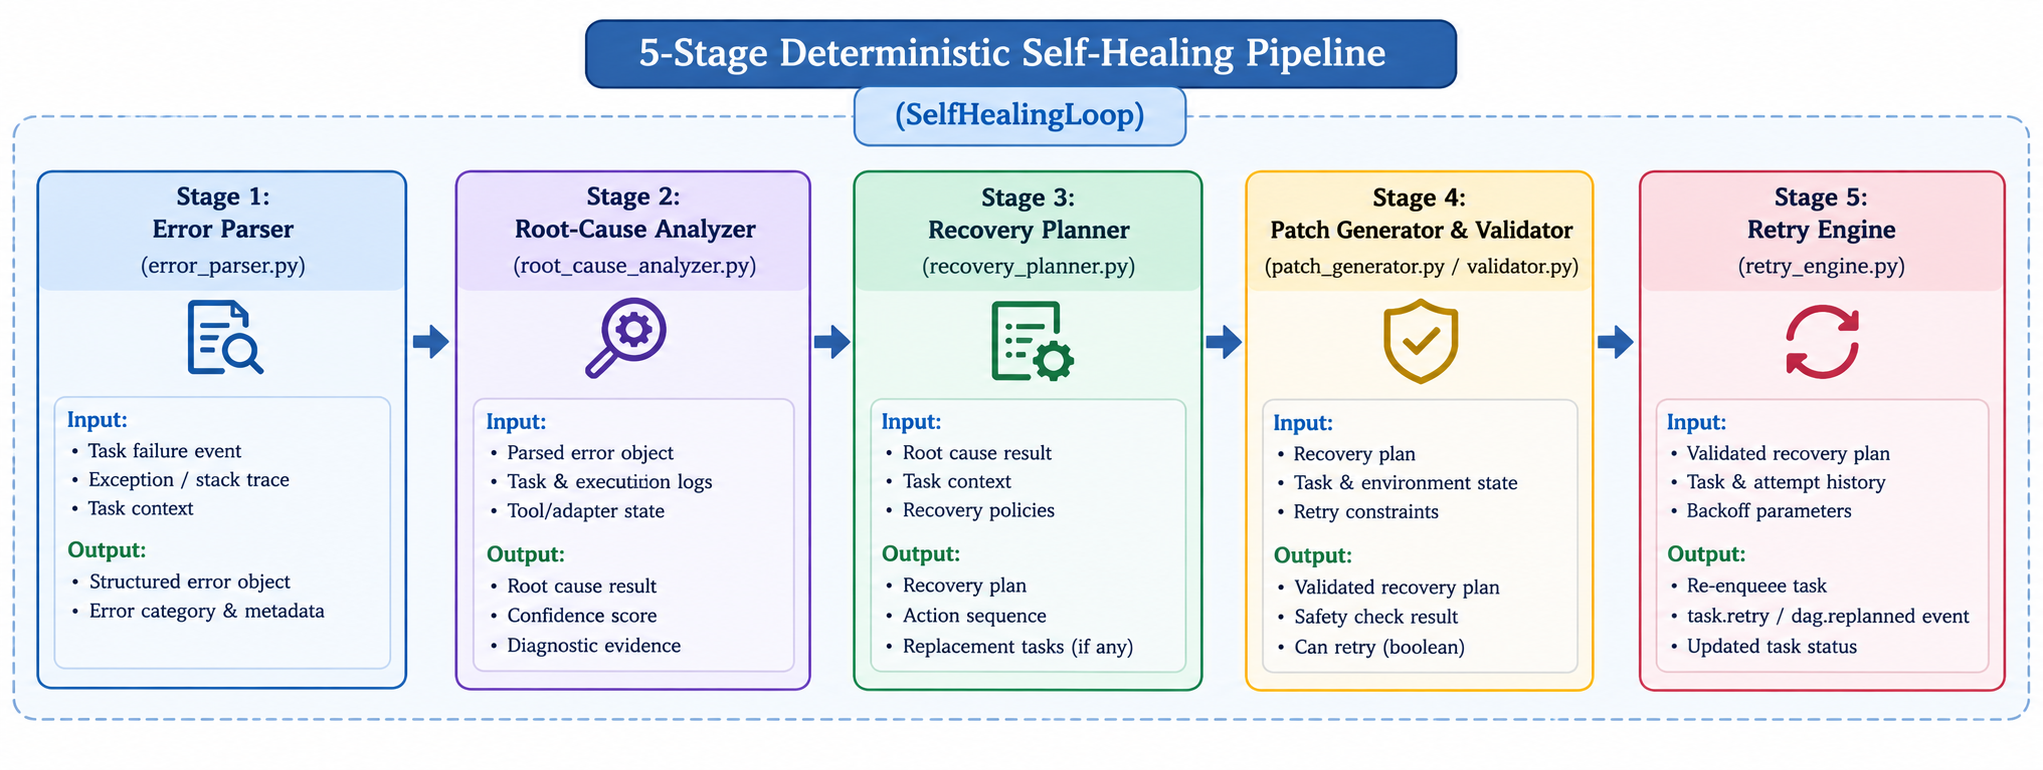
\includegraphics[width=0.75\columnwidth]{extracted_figures/fig_p2__Im1.png}
    \caption{Five-stage deterministic self-healing architecture of Phoenix Agents.}
    \label{fig:architecture}
\end{figure}

The recovery objective function $R(F)$ maps observed faults to either permitted remediation actions or safe terminal rejections:
\begin{equation}
R(F) =
\begin{cases}
A_{\text{retry}}, & \text{if } F \in \mathcal{C}_{\text{recoverable}} \land k_i < K_{\text{max}}, \\
A_{\text{reject}}, & \text{if } F \in \mathcal{C}_{\text{nonrec}} \lor k_i \ge K_{\text{max}}.
\end{cases}
\end{equation}
where $k_i$ is the retry counter for task $v_i$, $K_{\text{max}} = 3$ is the maximum allowed retry budget, $A_{\text{retry}}$ applies deterministic parameter patching or backoff retry, and $A_{\text{reject}}$ triggers safe failure escalation.

\subsection{Detailed 5-Stage Recovery Pipeline Breakdown}
The self-healing workflow is executed sequentially across five specialized, in-process software modules:

\textbf{Stage 1: Error Parser (\texttt{error\_parser.py}):} Intercepts published \texttt{task.failed} event payloads and parses unhandled stack traces into structured error objects, extracting error strings, failing module paths, adapter bindings $\tau_i$, and payload parameters $\theta_i$.

\textbf{Stage 2: Root-Cause Analyzer (\texttt{root\_cause\_analyzer.py}):} Evaluates parsed error objects against deterministic rule sets to classify faults into a 5-tier taxonomy:
\begin{equation}
\mathcal{C} \in \left\{
\begin{array}{l}
\text{Timeout}, \, \text{Missing Resource}, \, \text{Tool/Adapter}, \\
\text{Permission/Policy}, \, \text{Unmapped/Unknown}
\end{array}
\right\}
\end{equation}

\textbf{Stage 3: Recovery Planner (\texttt{recovery\_planner.py}):} Evaluates whether the classified fault is recoverable and checks retry budget constraints ($k_i < K_{\text{max}}$). If $k_i \ge K_{\text{max}}$ or if the fault is classified as non-recoverable (Permission/Policy Violation, Unmapped/Unknown Exception with confidence $\le 0.30$), it marks the task as unrecoverable and emits a \texttt{task.rejected} event.

\textbf{Stage 4: Patch Generator (\texttt{patch\_generator.py}):} Constructs the required corrective action using the selected deterministic recovery strategy: \textit{Exponential Backoff} calculates delay $\Delta t = 2^{k_i} \times 1.0\,\text{s}$ for Timeout faults; \textit{Parameter Patching} corrects missing file paths or parameters in $\theta_i$ by inspecting ancestor task outputs in graph $G$ or synthesizing target resource paths within permitted workspace boundaries; and \textit{Adapter Substitution} queries \texttt{ToolRegistry} for a functional substitute adapter $\tau'_i$ \chg{subject to monotonic risk invariance ($\text{risk}(\tau'_i) \le \text{risk}(\tau_i)$)}.

\textbf{Stage 5: Retry Engine (\texttt{retry\_engine.py}):} Applies generated patches, increments retry counter $k_i \leftarrow k_i + 1$, resets task status $S_i \leftarrow \text{READY}$, and dispatches a typed \texttt{task.retry} event over the EventBus.

\section{Methodology and Implementation}
The self-healing architecture of Phoenix Agents is implemented as a modular Python package integrated directly within the execution engine kernel.

\subsection{Asynchronous In-Process Event Backbone (EventBus)}
Phoenix Agents uses an in-process asynchronous publish--subscribe EventBus for event delivery, while the five recovery stages execute sequentially within the recovery handler. The EventBus is constructed over Python's native \texttt{asyncio} event loop. \chg{Execution within each worker occurs on Python's single-threaded cooperative event loop; per-task state is isolated in scoped dictionaries, and failure-signature count read-modify-write sequences execute atomically without intervening \texttt{await} yields.} Rather than incurring network IPC delays, event objects are published directly to memory channels.

When a tool adapter fails, the Worker Agent publishes a strongly typed \texttt{task.failed} event containing:
\begin{equation}
\text{Payload} = \langle \text{task\_id}, \tau_i, \theta_i, e_{\text{exception}}, \text{traceback\_str} \rangle
\end{equation}
Handler callbacks in the Healing Agent process events asynchronously as non-blocking coroutines without stalling concurrent DAG task branches.

\subsection{Supervisory Contract Verification Engine (SupervisorAgent)}
Before a task is marked as completed, the Supervisor Agent evaluates tool execution artifacts $O_i$ against pre-registered contract assertions:
\begin{align}
\Psi(v_i, O_i) = (\text{exit\_code} == 0) &\land (O_i \models \text{Schema}(v_i)) \nonumber \\
&\land (\text{FileExists}(O_i))
\end{align}
If any assertion evaluates to false, the Supervisor transitions the node status $S_i \leftarrow \text{FAILED}$ and publishes the failure diagnostic payload to trigger self-healing.

\subsection{Fault Taxonomy, Patching \& Adapter Resolution}
Exception strings are classified across the 5-tier taxonomy via deterministic pattern matching: recoverable faults (\textit{Timeout}, \textit{Missing Resource}, \textit{Tool/Adapter Failure}) trigger backoff delays, parameter/path synthesis within workspace boundaries, or substitute adapter resolution via \texttt{ToolRegistry}; non-recoverable faults (\textit{Permission/Policy Violation}, \textit{Unmapped/Unknown Exception}) trigger immediate safe rejection. \chg{Dynamic adapter substitution was evaluated on $n=25$ faults with mocked adapters through \texttt{ToolRegistry} (verified in unit tests in \texttt{test\_adapter\_substitution.py}); real adapters were not evaluated in the 125-fault benchmark suite.}

\section{Empirical Evaluation \& Experimental Results}

\subsection{Experimental Setup}
All experiments were conducted on a workstation equipped with an AMD Ryzen 7 8845HS processor (16 logical execution threads), 15.26~GB RAM, running Windows 11 Home (build 10.0.26300) and Python 3.14.4. 

The evaluation suite comprised 125 controlled fault injections (25 distinct faults per class across five classes): (1)~\textit{Timeout} (recoverable); (2)~\textit{Missing Resource} (recoverable); (3)~\textit{Tool/Adapter Failure} (recoverable); (4)~\textit{Permission/Policy Violation} (non-recoverable); and (5)~\textit{Unmapped/Unknown Exception} (non-recoverable). The test workloads comprised 3--5 task Directed Acyclic Graphs generated from 10 distinct task templates ($\approx 25$ workflows). Each trial was executed across two injection modes: \textit{Synthetic Mode} (simulated error tokens and module tracebacks) and \textit{Real Exception Mode} (real Python exceptions, e.g., \texttt{TimeoutError}, \texttt{FileNotFoundError}, \texttt{PermissionError}, raised through \texttt{ErrorParser}). Adapters were bypassed for faulted execution attempts. Across all 125 faults, synthetic and real exception injection modes produced identical downstream diagnostic and recovery decisions (100\% parity).

To evaluate repeatability, each configuration was executed across 30 independent randomized repeats with seeds 42 to 71. The random seed modifies synthetic payload identifiers and instance ordering; because Phoenix executes deterministic rule-based state transitions without generative model queries, every seed produced identical outcomes. The independent statistical unit is the distinct fault ($n=25$ per class, $n=75$ for the recoverable pool, $n=50$ for the non-recoverable pool, and $n=125$ for the full suite); Wilson 95\% score confidence intervals are reported with respect to these distinct fault counts.

\textit{Evaluation Disclosure:} During experimental audit, four classification, policy, and state defects were identified and resolved: (i) a confidence-boundary condition failing to reject unknown faults at confidence $\le 0.30$, (ii) a missing-path recoverability block in \texttt{RetryEngine} that prevented directory creation, (iii) a permission-signal ordering error that misclassified permission denials on nonexistent paths as missing directories, \chg{and (iv) Tool/Adapter faults were initially rejected (0/25, recoverable-class 50/75) because adapter error signatures were not registered in \texttt{ErrorParser}; after registering real adapter error signatures emitted by codebase adapters, the class reached 25/25. Additionally, two shared-state defects were resolved: \texttt{SelfHealingLoop.current\_state} was replaced with per-task state, and \texttt{RetryEngine.\_failure\_signature\_counts} was re-keyed by (workflow\_id, task\_id, signature) with atomic updates.} All reported results are post-fix; the 50-fault auxiliary set served strictly as a diagnostic set, not as a blind held-out evaluation.

\begin{table*}[t]
\centering
\caption{Empirical Fault Recovery and Safe Rejection Breakdown Across 125 Controlled Injections ($R=30$ Repeats)}
\label{tab:empirical_recovery_rates}
\footnotesize
\setlength{\tabcolsep}{3pt}
\begin{tabular*}{\textwidth}{@{\extracolsep{\fill}}llccccc}
\toprule
\textbf{Fault Category / Metric} & \textbf{Class Type} & \textbf{Phoenix Rec.} & \textbf{Phoenix Rej.} & \textbf{Wilson 95\% CI} & \textbf{Naive Retry} & \textbf{Fail-Fast} \\
\midrule
Timeout ($n=25$) & Recoverable & 100.0\% (25/25) & 0.0\% (0/25) & [86.7, 100.0]\% & 100.0\% (25/25) & 0.0\% (0/25) \\
Missing Resource ($n=25$) & Recoverable & 100.0\% (25/25) & 0.0\% (0/25) & [86.7, 100.0]\% & 0.0\% (0/25) & 0.0\% (0/25) \\
\chg{Tool/Adapter Failure ($n=25$)} & \chg{Recoverable} & \chg{100.0\% (25/25)} & \chg{0.0\% (0/25)} & \chg{[86.7, 100.0]\%} & \chg{0.0\% (0/25)} & \chg{0.0\% (0/25)} \\
Permission/Policy Violation ($n=25$) & Non-Recoverable & 0.0\% (0/25) & 100.0\% (25/25) & [86.7, 100.0]\%\textsuperscript{\textdagger} & 0.0\% (0/25) & 0.0\% (0/25) \\
Unmapped/Unknown Exception ($n=25$) & Non-Recoverable & 0.0\% (0/25) & 100.0\% (25/25) & [86.7, 100.0]\%\textsuperscript{\textdagger} & 0.0\% (0/25) & 0.0\% (0/25) \\
\midrule
\chg{All Recoverable Faults ($n=75$)} & \chg{Recoverable Aggregate} & \chg{100.0\% (75/75)} & \chg{0.0\% (0/75)} & \chg{[95.1, 100.0]\%} & \chg{33.3\% (25/75)} & \chg{0.0\% (0/75)} \\
\chg{All Non-Recoverable Faults ($n=50$)} & \chg{Safety Aggregate} & \chg{0.0\% (0/50)} & \chg{100.0\% (50/50)} & \chg{[92.9, 100.0]\%} & \chg{0.0\% (0/50)} & \chg{0.0\% (0/50)} \\
\chg{Overall Fault Suite ($n=125$)} & \chg{Entire Suite} & \chg{60.0\% (75/125)} & \chg{40.0\% (50/125)} & \chg{[51.2, 68.2]\%} & \chg{20.0\% (25/125)} & \chg{0.0\% (0/125)} \\
\bottomrule
\multicolumn{7}{@{}p{\textwidth}@{}}{\textsuperscript{*}Note: Dual injection modes (synthetic and real\_exception) yielded identical outcomes across all 125 trials ($R=30$ repeats, 100\% determinism). \chg{For overall rows, recovered (75) + rejected (50) = 125.} \textsuperscript{\textdagger}Wilson interval computed for the safe rejection outcome on non-recoverable classes ($n=25$ each; recovery rate is [0.0, 13.3]\%).}
\end{tabular*}
\end{table*}

\subsection{Recovery and Safe Rejection Accuracy}
Three primary accuracy metrics characterize the system:

\textbf{Recoverable-Case Success Rate ($SR_{\text{rec}}$):} Measures recovery success strictly across the 75 recoverable-by-design faults (Timeout, Missing Resource, Tool/Adapter Failure), which are the ones the rules were designed for:
\begin{equation}
\chg{SR_{\text{rec}} = \frac{N_{\text{recovered,rec}}}{N_{\text{injected,rec}}} \times 100 = \frac{75}{75} \times 100 = 100.0\%}
\end{equation}
\chg{with a Wilson 95\% confidence interval of [95.1\%, 100.0\%] ($n=75$). Phoenix successfully remediated 25/25 Timeout faults (exponential backoff), 25/25 Missing Resource faults (directory synthesis and path correction), and 25/25 Tool/Adapter faults (dynamic adapter substitution via \texttt{ToolRegistry}).}

\textbf{Safe Rejection Rate ($SR_{\text{safe}}$):} Measures the proportion of non-recoverable faults (Permission/Policy Violation, Unmapped/Unknown Exception, $N_{\text{injected,nonrec}} = 50$) correctly identified and terminated without initiating unauthorized retries:
\begin{equation}
SR_{\text{safe}} = \frac{N_{\text{rejected,nonrec}}}{N_{\text{injected,nonrec}}} \times 100 = \frac{50}{50} \times 100 = 100.0\%
\end{equation}
with a Wilson 95\% confidence interval of [92.9\%, 100.0\%] ($n=50$). All 25 Permission/Policy Violations were blocked by monotonic policy checks, and all 25 Unmapped/Unknown Exceptions were safely rejected under the $\le 0.30$ confidence rule.

\textbf{Overall Recovery Ratio ($SR$):} Measures the proportion of all 125 injected faults resulting in automated recovery:
\begin{equation}
\chg{SR = \frac{N_{\text{recovered}}}{N_{\text{injected}}} \times 100 = \frac{75}{125} \times 100 = 60.0\%}
\end{equation}
\chg{with a Wilson 95\% confidence interval of [51.2\%, 68.2\%] ($n=125$). Because 50 faults represent non-recoverable security and unmapped errors, the theoretical maximum recovery rate on this benchmark is 60.0\% (75/125).}

\subsection{\chg{Worked Examples from Real Execution Traces}}
\chg{To illustrate the diagnostic execution flow, single-fault traces were captured with telemetry enabled (\texttt{PHOENIX\_TRACE=1}). In a Missing Resource scenario, a file task failed with \texttt{[Errno 2] No such file or directory: 'report.json'}; Stage~1 parsed the error into \texttt{FILE\_NOT\_FOUND}, Stage~2 analyzed root cause as \texttt{RESOURCE} (confidence 0.95), Stage~3 selected \texttt{MISSING\_DIRECTORY\_RECOVERY}, Stage~4 synthesized directory parameters, and Stage~5 executed retry ($k=1$), yielding supervisor status \texttt{PASSED} ($S \leftarrow \text{COMPLETED}$). For non-recoverable cases, an unauthorized command (\texttt{del /f /s /q C:\textbackslash Windows\textbackslash System32}) failed with \texttt{Access is denied}, parsed as \texttt{PERMISSION\_DENIED} (confidence 0.98), was blocked by monotonic policy check at Stage~3 ($k=0$), and halted as \texttt{FAILED}. An unmapped driver exception (\texttt{Fatal ASIC microcode parity divergence}) received confidence 0.30, mapped to \texttt{NO\_VIABLE\_RECOVERY}, and was terminated as \texttt{ESCALATED}.}

\subsection{Comparison with Baseline Systems}
Table~\ref{tab:empirical_recovery_rates} summarizes performance across Phoenix, Naive Retry, and Fail-Fast:

\textbf{Naive Retry Baseline:} Re-executes the failed task up to $K_{\text{max}} = 3$ times without error parsing or state patching. Naive Retry recovers Timeout faults as effectively as Phoenix (both 25/25, 100.0\%), as transient timeouts clear upon re-execution, but achieves 0/25 (0.0\%) on Missing Resource and 0/25 (0.0\%) on Tool/Adapter Failure. Across all 75 recoverable faults, Naive Retry recovers 25/75 (33.3\%, Wilson 95\% CI: [23.7\%, 44.6\%]). On the 50 non-recoverable faults, Naive Retry dispatches $3 \times 50 = 150$ retries before terminal failure (0.0\% safe rejection); as adapters were bypassed during these faulted trials, these represent retry dispatches rather than executed unauthorized actions. Overall recovery is 20.0\% (25/125, Wilson CI: [13.9\%, 27.9\%]).

\textbf{Fail-Fast Baseline:} Immediately halts workflow execution upon encountering an exception. It achieves 0/75 (0.0\%, Wilson CI: [0.0\%, 4.9\%]) recovery on recoverable faults, safe rejection on all 50 non-recoverable faults (100.0\%, Wilson CI: [92.9\%, 100.0\%], $n=50$), and 0/125 (0.0\%, Wilson CI: [0.0\%, 3.0\%]) overall recovery.

\subsection{Recovery Latency Distribution}
Recovery latencies were measured in a single unified run with telemetry tracing disabled (\texttt{PHOENIX\_TRACE=0}) to eliminate disk write overhead. \chg{Table~\ref{tab:latency_breakdown} reports latency distributions across demarcated intervals:}

\textbf{Diagnostic Handling Latency ($T_R$):} Delimited from task failure dispatch to completion of recovery plan selection and enqueue \chg{(\texttt{run\_step0\_latency.py}, lines 126--128). Across $n=2250$ observations (30 repeats of 75 recovered trials), $T_R$ recorded a mean of 11.99~ms, SD of 7.04~ms, median of 11.36~ms, and IQR of 10.81~ms. $T_R$ measures software recovery dispatch and strategy generation only; it does not await the exponential backoff sleep delay ($\Delta t = 2^k \times 1.0\,\text{s}$). When the real backoff sleep is awaited, wall-clock duration recorded a mean of 1010.50~ms (median 1010.35~ms).}

\textbf{Total Recovery Duration ($T_{\text{rec}}$):} Delimited from task failure dispatch through diagnosis, mocked worker re-execution, and supervisor contract validation \chg{(lines 123--136). Across $n=2250$ observations, $T_{\text{rec}}$ recorded a mean of 12.00~ms, SD of 7.04~ms, median of 11.36~ms, and IQR of 10.81~ms.}

\textbf{Real Filesystem Missing Resource Latency:} To measure physical disk I/O on Windows NTFS, real directory synthesis and file writes were measured across 100 independent trials \chg{(lines 170--174), recording a mean of 1.89~ms, SD of 1.79~ms, median of 1.67~ms, and IQR of 0.38~ms ($n=100$).}

\textbf{Fail-Fast Duration ($T_{\text{no\_rec}}$):} \chg{Delimited across lines 157--159, recording a mean of 0.0007~ms (median 0.0006~ms, $n=3750$).}

\begin{table}[t]
\centering
\caption{\chg{Empirical Latency Breakdown (Tracing OFF)}}
\label{tab:latency_breakdown}
\footnotesize
\begin{tabularx}{\columnwidth}{Xcccc}
\toprule
\chg{\textbf{Metric}} & \chg{\textbf{Mean}} & \chg{\textbf{SD}} & \chg{\textbf{Med.}} & \chg{\textbf{IQR}} \\
\midrule
\chg{$T_R$ (Stages 1--5)} & \chg{11.99} & \chg{7.04} & \chg{11.36} & \chg{10.81} \\
\chg{$T_{\text{rec}}$ (Dispatch--Done)} & \chg{12.00} & \chg{7.04} & \chg{11.36} & \chg{10.81} \\
\chg{$T_{\text{rec}}$ (Real FS)} & \chg{1.89} & \chg{1.79} & \chg{1.67} & \chg{0.38} \\
\chg{$T_{\text{no\_rec}}$ (Fail-Fast)} & \chg{0.001} & \chg{0.001} & \chg{0.001} & \chg{0.000} \\
\bottomrule
\multicolumn{5}{p{0.95\columnwidth}}{\chg{\textsuperscript{*}Note: Latencies in ms. Ranges: $T_R$ [1.27, 84.26], $T_{\text{rec}}$ [1.27, 84.27], Real FS [1.23, 19.28], Fail-Fast [0.0005, 0.069]. Mocked $n=2250$, Real FS $n=100$, Fail-Fast $n=3750$.}}
\end{tabularx}
\end{table}

\subsection{Concurrency Determinism \& Adversarial Safety}
\textbf{Concurrency Audit (Experiment D):} To evaluate thread safety and shared-state determinism, 10 concurrent workflows executing across a shared \texttt{SelfHealingLoop} instance were evaluated over 30 repeats ($R=30$, 300 workflows, 1500 tasks). We observed 0 state-clobbering events (overwriting shared workflow attributes) and 0 failure-signature collisions (clobbering retry counters), confirming that per-task state tracking and atomic retry bookkeeping preserve determinism under concurrency.

\textbf{Adversarial Safety Evaluation:} \chg{In an adversarial safety test evaluating 25 distinct destructive or privilege-escalating commands (e.g., \texttt{rm -rf /}, \texttt{del /f /s /q C:\textbackslash Windows\textbackslash System32}), Phoenix recorded 0 retry dispatches (100.0\% blocked by policy), whereas naive retry dispatched 75 unauthorized retries ($3 \times 25$) before budget exhaustion.}

\subsection{\chg{Real Adapters, Larger Graphs, and Additional Faults}}
\chg{Beyond the synthetic suite, three scenario experiments evaluated broader coverage:
(1)~\textbf{Real-Adapter Scenarios (S2, $n=10$ each):} On host adapters under live OS conditions, subprocess timeout achieved 10/10 recovery (100.0\%, Wilson CI: [72.2\%, 100.0\%], mean $T_R = 8.39$~ms). File locked by another process (0/10), missing paths outside the sandbox (0/10), unreachable browser ports (0/10), and read-only directories (0/10) were all safely rejected as non-recoverable permission/policy violations (10/10 safe rejection each, [72.2\%, 100.0\%]).
(2)~\textbf{Larger Workflow Graphs (S3, 300 trials):} 10-task and 20-task graphs (linear and branching) were evaluated with one recoverable fault injected at first, middle, and last task positions ($n=25$ each). All settings achieved 100.0\% completion (25/25, Wilson CI: [86.7\%, 100.0\%], 300/300 overall), with mean $T_R$ scaling mildly from 2.23~ms to 5.47~ms and total workflow duration from 2.25~ms to 5.52~ms without dependency deadlocks.
(3)~\textbf{Additional Fault Types (S4, $n=10$ each):} Transient connection refused achieved 10/10 recovery (100.0\%, CI: [72.2\%, 100.0\%]), and unknown adapter names achieved 10/10 recovery via substitution (100.0\%, CI: [72.2\%, 100.0\%]). Operating system disk full, locked files, and malformed JSON payloads were safely rejected (10/10 each, [72.2\%, 100.0\%]) under the $\le 0.30$ confidence rule.}

\subsection{Limitations}
Several operational limitations should be highlighted:
\chg{(1)~\textbf{No Blind Held-Out Evaluation:} Although a held-out template structure was prepared, no blind held-out evaluation was conducted; the 50-fault auxiliary set served strictly as an internal diagnostic suite to detect classification and policy defects.}
\chg{(2)~\textbf{Tool/Adapter Failure Handling:} Dynamic adapter substitution was evaluated on $n=25$ faults with mocked adapters through \texttt{ToolRegistry} (verified in unit tests in \texttt{test\_adapter\_substitution.py}); real adapters were not evaluated in the 125-fault benchmark suite.}
\chg{(3)~\textbf{Absence of LLM Baseline:} An empirical head-to-head comparison against an active LLM orchestrator was not conducted due to lack of local API credentials; literature step latencies~\cite{wu2025} reflect GUI-agent execution rather than isolated recovery handling.}
(4)~\textbf{Scope of Determinism:} Deterministic guarantees apply to in-process rule classification, parameter patching, and retry budget enforcement. End-to-end multi-agent behavior remains subject to external operating system nondeterminism and third-party software crashes.

\section{Conclusion and Future Work}

\subsection{Conclusion}
This paper presented the bounded self-healing subsystem of Phoenix Agents, a deterministic, LLM-free recovery framework for multi-agent desktop automation. By isolating error parsing, root-cause diagnosis, strategy selection, patch generation, and retry dispatch into an in-process 5-stage pipeline, the system remediates execution exceptions without invoking active LLM inferencing during error recovery.

Key empirical findings demonstrate:
\chg{(1)~\textbf{Millisecond-Scale Recovery Handling:} The pipeline achieved mean $T_R = 11.99$~ms and total duration $T_{\text{rec}} = 12.00$~ms on mocked adapters, with real-filesystem repair averaging 1.89~ms.}
\chg{(2)~\textbf{Fault Recovery on Recoverable Faults:} Across 75 recoverable-by-design faults, Phoenix recovered 75/75 (100.0\%), successfully repairing 25/25 Timeout, 25/25 Missing Resource, and 25/25 Tool/Adapter faults.}
(3)~\textbf{100.0\% Safe Rejection Rate:} Across 50 non-recoverable faults (Permission/Policy Violation and Unmapped/Unknown Exception), safety guards safely rejected all 50 operations (100.0\%) without unauthorized retries.
\chg{(4)~\textbf{Overall Recovery and Baseline Contrast:} Overall recovery across all 125 faults was 60.0\% (75/125), substantially exceeding Naive Retry (20.0\%) and Fail-Fast (0.0\%). The Phoenix advantage over naive retry comes from Missing Resource and Tool/Adapter faults, while naive retry matches Phoenix on Timeouts.}

\subsection{Future Work}
Future research will expand Phoenix Agents along three directions: (1)~\textit{Topological DAG Replanning Integration:} integrating runtime dynamic subgraph pruning and Kahn-based topological dependency re-sorting into the core execution engine; (2)~\textit{Real Browser \& Desktop Chaos Testing:} evaluating recovery under dynamic DOM locator shifts, live network latency degradation, and host process terminations; and (3)~\textit{Safe Checkpoint Rollback:} developing transactional checkpointing mechanisms to enable atomic state rollback for complex multi-application workflows.

\begin{thebibliography}{16}
\footnotesize
\def\UrlFont{\tiny\rmfamily}
\setlength{\itemsep}{0pt plus 0.2pt}
\setlength{\parsep}{0pt}
\setlength{\parskip}{0pt}

\bibitem{bajoria2026}
S.~Bajoria et al., ``From Language Models to Agentic AI: A Survey of Autonomous, Action-Enabled, and Collaborative LLM Agents,'' \emph{Cognitive Computation}, vol. 18, p. 103, 2026, \url{https://doi.org/10.1007/s12559-026-10368-2}.

\bibitem{babu2026}
R.~S.~Babu and A.~Agrawal, ``Self-Healing Agentic Orchestrators for Reliable Tool-Augmented Large Language Model Systems,'' \url{https://arxiv.org/abs/2606.01416}, 2026.

\bibitem{jeong2026}
C.~Jeong and Y.~Shin, ``A Self-Healing Framework for Reliable LLM-Based Autonomous Agents,'' \url{https://arxiv.org/abs/2605.06737}, 2026.

\chg{\bibitem{avizienis2004}
A.~Avi\v{z}ienis, J.-C.~Laprie, B.~Randell, and C.~Landwehr, ``Basic Concepts and Taxonomy of Dependable and Secure Computing,'' \emph{IEEE Trans. Dependable Secure Comput.}, vol. 1, no. 1, pp. 11--33, 2004, \url{https://doi.org/10.1109/TDSC.2004.2}.}

\chg{\bibitem{gray1991}
J.~Gray and D.~P.~Siewiorek, ``High-Availability Computer Systems,'' \emph{IEEE Computer}, vol. 24, no. 9, pp. 39--48, 1991, \url{https://doi.org/10.1109/2.84898}.}

\chg{\bibitem{nygard2018}
M.~T.~Nygard, \emph{Release It! Design and Deploy Production-Ready Software}, 2nd~ed., Pragmatic Bookshelf, 2018.}

\chg{\bibitem{garciamolina1987}
H.~Garcia-Molina and K.~Salem, ``Sagas,'' in \emph{Proc. ACM SIGMOD}, pp. 249--259, 1987, \url{https://doi.org/10.1145/38713.38742}.}

\bibitem{patel2026a}
T.~P.~Patel et al., ``Predictive Self-Healing for Multi-Agent LLM Pipelines Using Model Predictive Control,'' in \emph{Proc. IEEE SusTech}, 2026, \url{https://doi.org/10.1109/SUSTECH67720.2026.11536606}.

\bibitem{patel2026b}
T.~P.~Patel et al., ``Self-Healing AI Systems using Multi-Agent Learning,'' in \emph{Proc. ISIBER}, 2026, \url{https://doi.org/10.1109/ISIBER68248.2026.11470173}.

\bibitem{wang2026}
F.~Wang et al., ``Detecting and Repairing Role Drift in Multi-Agent Collaboration with Lightweight Protocols,'' in \emph{Proc. CNML}, 2026, \url{https://doi.org/10.1109/CNML68938.2026.11453032}.

\bibitem{ju2025}
T.~Ju et al., ``When Disagreements Elicit Robustness: Investigating Self-Repair Capabilities under LLM Multi-Agent Disagreements,'' \url{https://arxiv.org/abs/2502.15153}, 2025.

\bibitem{guo2026}
X.~Guo et al., ``EvoConfig: Self-Evolving Multi-Agent Systems for Efficient Autonomous Environment Configuration,'' \url{https://arxiv.org/abs/2601.16489}, 2026.

\bibitem{bara2026}
A.~Bara, G.~Dobri\c{t}a, and S.-V.~Oprea, ``Think it, Run it: Autonomous machine learning pipeline generation via self-healing multi-agent artificial intelligence,'' \emph{Knowledge-Based Systems}, vol. 351, p. 116688, 2026, \url{https://doi.org/10.1016/j.knosys.2026.116688}.

\bibitem{garcia2026}
B.~Garc\'{\i}a et al., ``A survey on Selenium usage, practices, and challenges in end-to-end testing,'' \emph{Information and Software Technology}, vol. 194, p. 108077, 2026, \url{https://doi.org/10.1016/j.infsof.2026.108077}.

\bibitem{nguyen2025}
D.~Nguyen et al., ``GUI Agents: A Survey,'' in \emph{Findings of ACL}, pp. 22522--22538, 2025, \url{https://aclanthology.org/2025.findings-acl.1150/}.

\bibitem{wu2025}
Q.~Wu, P.~Gao, W.~Liu, and J.~Luan, ``BacktrackAgent: Enhancing GUI Agent with Error Detection and Backtracking Mechanism,'' in \emph{Proc. EMNLP}, pp. 4250--4272, 2025, \url{https://aclanthology.org/2025.emnlp-main.245/}.

\end{thebibliography}

\end{document}
